\chapter{RESEARCH APPROACH}
\section{PROV-PUB-O: a provenance ontology for research publications}
This section presents the approach to the creation of an ontology for capturing provenance in the process of preparing research publications. The ontology is divided into two parts. 

The first part --- Section~\ref{subsec:structure} --- describes the structure of a research publication. We base our work on the Document Components Ontology (DoCO), which is one of the Semantic Publishing and Referencing Ontologies (SPAR). SPAR focuses a lot on modeling citations and bibliographic references. Four out of the eight ontologies in SPAR deal with citations and bibliographic references. (They are CiTO, the Citation Typing Ontology, FaBiO, the FRBR-aligned Bibliographic Ontology, BiRO, the Bibliographic Reference Ontology, and C4O, the Citation Counting and Context Characterization Ontology.) So SPAR is good for modeling the linkage between publications. 

In this thesis we focus on the reproducibility of a certain publication, so we do not delve deep into citations and bibliographic references as they have nothing to do with the computational experiments presented in the current publication. 

We model the structure of a research publication because experimental results must reside somewhere in the publication. Textual elements in the publication provide contextual information and explanation for the reported results. Although these elements are not parts of the process leading to the reported results, they are documentation that help readers to correctly interpret the results, so we include structural elements of research publications in the provenance.

The second part --- Section~\ref{subsec:process} --- describes the process leading to the reported results. It is a specialization of the W3C Provenance Ontology (PROV-O) for the use case of research publication preparation. We base the development of PROV-PUB-O on PROV-O because using general provenance ontologies such as PROV-O proves to be an effective way to keep track of the lineage of the source data and the changing processes leading to the final results. 

The goal of the specialization is to make the specialized ontology, namely PROV-PUB-O, detailed enough to enable the creation of \emph{executable provenance graphs} (EPGs). In an EPG, the semantics of each element in the process leading to the reported results is well defined, so the replication of the process becomes straightforward. Moreover, the process described with an EPG can even be used to validate the scientific conclusions by allowing readers to adapt the experiment reported in the paper and carry out their own studies.

The hypothesis to justify for PROV-PUB-O is that it is useful in the use case of modeling research publication preparation process in the domain of earth science for the purpose of replicating data transformation processes and validating scientific conclusions. We would like to show that less effort is required to create EPGs with PROV-PUB-O than with PROV-O. We will cover the measurement of effort amount and the details of the benchmark modeling tasks in Section~\ref{subsec:evaluation}.

\subsection{Publication structure modeling}
\label{subsec:structure}
Document structure models such as the Document Components Ontology (DoCO)\footnote{DoCO, the Document Components Ontology: http://purl.org/spar/doco} are usually based on structural patterns \cite{di2014dealing} and rhetorical structure theory (RST) \cite{taboada2006rhetorical}.

Here we take DoCO as an example. DoCO defines structural (e.g. block, inline, paragraph, section, chapter, etc. --- meaning what the component looks like) as well as rhetorical (e.g. introduction, discussion, acknowledgements, reference list, figure, appendix, etc. --- meaning what role the component plays in the document) document components.

Figure~\ref{fig:doco} shows the components of DoCO and the respective classes included in these components.
\begin{figure}[h]
	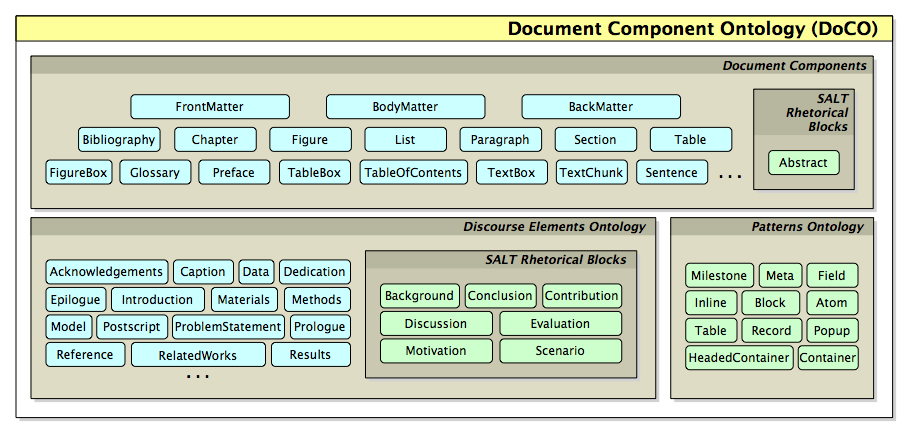
\includegraphics[width=\textwidth]{doco-architecture.png}
	\caption{Architecture of DoCO, the Document Components Ontology}
	\label{fig:doco}
\end{figure}

Structural document component types are closely related to the typesetting of the component contents. For example, if a block of text consisting of a title and several paragraphs is known to be a chapter, then at the time of rendering this block, the title can be made larger, proper font and size can be set for the content paragraphs, and the proper spacing can be set between this block and the blocks previous and next to it. Therefore, each structural document component type is like a class used to label HTML elements, and to be rendered according to class styles defined in Cascading Style Sheets (CSS).

Rhetorical document component types are completely irrelevant to typesetting --- just knowing a block of text is an ``introduction'' has nothing to do with properly formatting it. Rather, rhetorical types focus on the \emph{relations} between document parts, so these types are actually \emph{types of relations}. For example, the ``introduction'' component of a paper is usually a chapter, but theoretically it can be a section or even just a paragraph, leading to very different typesetting options. But just look at how we call this ``introduction'' component -- we call it ``introduction \emph{of} a paper'', i.e., an introduction component is always \emph{of something}. It does not make sense to have a ``floating'' introduction attached to nothing. 

In light of this relational perspective of rhetorical types, we make the following changes from DoCO:

\begin{itemize}
	\item The sro:Abstract class is changed to the pub:abstract property, whose domain is (doco:Chapter or doco:Section) and (dcterms:isPartOf some doco:BodyMatter or doco:FrontMatter), and range is pub:Document. The prefix sro expands to http://salt.semanticauthoring.org/ontologies/sro\# and stands for SALT (Semantically Annotated \LaTeX \cite{groza2007salt}) Rhetorical Ontology. The prefix doco expands to http://purl.org/spar/doco/, and the prefix dcterms expands to http://purl.org/dc/terms/, meaning DCMI (Dublin Core$^{\textregistered}$ Metadata Initiative) Metadata Terms\footnote{DCMI Metadata Terms: http://dublincore.org/documents/dcmi-terms/}. Finally, the prefix pub is for PROV-PUB-O, which is under development and not published yet.
	\item The sro:Background class is changed to the pub:background property, whose domain is (doco:Chapter or doco:Section) and (dcterms:isPartOf some doco:BodyMatter), and range is pub:Document. 
	\item Classes sro:Conclusion, sro:Contribution, sro:Discussion, sro:Evaluation, sro:Motivation, sro:Scenario are changed in the same manner as sro:Background. Note that these classes are different from sro:Abstract in that they cannot be part of the front matter component of a document.
	\item The class deo:Acknowledgements \comment{not sure yet.} The prefix deo here expands to http://purl.org/spar/deo/ and stands for the Discourse Elements Ontology\footnote{The Discourse Elements Ontology: http://purl.org/spar/deo}.
\end{itemize}

The hypotheses to justify here is that properties are more useful than rhetorical concepts in DoCO, the Document Components Ontology, in describing publication components. ("abs a Section; isAbstractOf article" vs. "abs a Abstract; isPartOf article.")

\subsection{Result generating process modeling}
\label{subsec:process}
Hypotheses to justify: PROV-PUB-O is more useful than PROV-O in the use case.

Subproperties of prov:wasAssociatedWith are more useful than itself in the use case.

\subsection{Model evaluation approach}
\label{subsec:evaluation}

\section{Automatic provenance capturing mechanism} 
VisTrails \cite{freire2014reproducibility}
Architecture for provenance systems \cite{groth2006architecture}

Hypotheses to justify: Capturing provenance with this mechanism is more useful than capturing provenance with the workflow systems.

\comment{Compare Groth's architecture with the proposed mechanism}

\section{A proof-of-concept platform}
Hypotheses:

3: The implemented platform satisfies the requirements indicated by the mechanism.

3.1: The platform does not require explicit input from authors to capture provenance for research publications.

3.2: The platform is more useful than workflow systems for carrying out operations in research publication preparation process.

3.3: The platform captures sufficient provenance for replicating research publications.

%\resetfootnote %this command starts footnote numbering with 1 again.

%\begin{figure}
%\centering
%\vspace{2.0in}
%\caption[A Shorter Caption for the List of Figures]
%   {This is the Caption for the First Figure in Chapter 2.  It is a
%    long, long caption; we do not want to put the whole thing in the
%    List of Figures. A Shorter Caption can go in the square brackets.}
% If you like additional lines in the caption indented, see the root template
% file rpithes.tex for an example of using the caption package to do this.
%\end{figure}
 
%This is shown in table~\ref{mytable}.  % see \label below
 
%\begin{table}
%\caption{This is the Caption for Table 2}
%\label{mytable}        % \label command must always comes AFTER the caption
%\begin{center}
%\begin{tabular}{lll}
%Here's       & another     & example  \\
%of           & a           & table    \\
%floated      & with        & the      \\
%\verb+table+ & environment & command.
%\end{tabular}
%\end{center}
%\end{table}


%\section{This is a Section Heading}
 
%\subsection{This is a Subsection Heading} 
 
%Text before a footnote.\footnote{Here's the text of the footnote.}
%Text after the footnote.


%%% Local Variables: 
%%% mode: latex
%%% TeX-master: t
%%% End: 
